\PassOptionsToPackage{unicode=true}{hyperref} % options for packages loaded elsewhere
\PassOptionsToPackage{hyphens}{url}
%
\documentclass[]{book}
\usepackage{lmodern}
\usepackage{amssymb,amsmath}
\usepackage{ifxetex,ifluatex}
\usepackage{fixltx2e} % provides \textsubscript
\ifnum 0\ifxetex 1\fi\ifluatex 1\fi=0 % if pdftex
  \usepackage[T1]{fontenc}
  \usepackage[utf8]{inputenc}
  \usepackage{textcomp} % provides euro and other symbols
\else % if luatex or xelatex
  \usepackage{unicode-math}
  \defaultfontfeatures{Ligatures=TeX,Scale=MatchLowercase}
\fi
% use upquote if available, for straight quotes in verbatim environments
\IfFileExists{upquote.sty}{\usepackage{upquote}}{}
% use microtype if available
\IfFileExists{microtype.sty}{%
\usepackage[]{microtype}
\UseMicrotypeSet[protrusion]{basicmath} % disable protrusion for tt fonts
}{}
\IfFileExists{parskip.sty}{%
\usepackage{parskip}
}{% else
\setlength{\parindent}{0pt}
\setlength{\parskip}{6pt plus 2pt minus 1pt}
}
\usepackage{hyperref}
\hypersetup{
            pdftitle={Fundamentals of Mathematics and Statistics with R},
            pdfauthor={Dr.~Priyanga D. Talagala},
            pdfborder={0 0 0},
            breaklinks=true}
\urlstyle{same}  % don't use monospace font for urls
\usepackage{color}
\usepackage{fancyvrb}
\newcommand{\VerbBar}{|}
\newcommand{\VERB}{\Verb[commandchars=\\\{\}]}
\DefineVerbatimEnvironment{Highlighting}{Verbatim}{commandchars=\\\{\}}
% Add ',fontsize=\small' for more characters per line
\usepackage{framed}
\definecolor{shadecolor}{RGB}{248,248,248}
\newenvironment{Shaded}{\begin{snugshade}}{\end{snugshade}}
\newcommand{\AlertTok}[1]{\textcolor[rgb]{0.94,0.16,0.16}{#1}}
\newcommand{\AnnotationTok}[1]{\textcolor[rgb]{0.56,0.35,0.01}{\textbf{\textit{#1}}}}
\newcommand{\AttributeTok}[1]{\textcolor[rgb]{0.77,0.63,0.00}{#1}}
\newcommand{\BaseNTok}[1]{\textcolor[rgb]{0.00,0.00,0.81}{#1}}
\newcommand{\BuiltInTok}[1]{#1}
\newcommand{\CharTok}[1]{\textcolor[rgb]{0.31,0.60,0.02}{#1}}
\newcommand{\CommentTok}[1]{\textcolor[rgb]{0.56,0.35,0.01}{\textit{#1}}}
\newcommand{\CommentVarTok}[1]{\textcolor[rgb]{0.56,0.35,0.01}{\textbf{\textit{#1}}}}
\newcommand{\ConstantTok}[1]{\textcolor[rgb]{0.00,0.00,0.00}{#1}}
\newcommand{\ControlFlowTok}[1]{\textcolor[rgb]{0.13,0.29,0.53}{\textbf{#1}}}
\newcommand{\DataTypeTok}[1]{\textcolor[rgb]{0.13,0.29,0.53}{#1}}
\newcommand{\DecValTok}[1]{\textcolor[rgb]{0.00,0.00,0.81}{#1}}
\newcommand{\DocumentationTok}[1]{\textcolor[rgb]{0.56,0.35,0.01}{\textbf{\textit{#1}}}}
\newcommand{\ErrorTok}[1]{\textcolor[rgb]{0.64,0.00,0.00}{\textbf{#1}}}
\newcommand{\ExtensionTok}[1]{#1}
\newcommand{\FloatTok}[1]{\textcolor[rgb]{0.00,0.00,0.81}{#1}}
\newcommand{\FunctionTok}[1]{\textcolor[rgb]{0.00,0.00,0.00}{#1}}
\newcommand{\ImportTok}[1]{#1}
\newcommand{\InformationTok}[1]{\textcolor[rgb]{0.56,0.35,0.01}{\textbf{\textit{#1}}}}
\newcommand{\KeywordTok}[1]{\textcolor[rgb]{0.13,0.29,0.53}{\textbf{#1}}}
\newcommand{\NormalTok}[1]{#1}
\newcommand{\OperatorTok}[1]{\textcolor[rgb]{0.81,0.36,0.00}{\textbf{#1}}}
\newcommand{\OtherTok}[1]{\textcolor[rgb]{0.56,0.35,0.01}{#1}}
\newcommand{\PreprocessorTok}[1]{\textcolor[rgb]{0.56,0.35,0.01}{\textit{#1}}}
\newcommand{\RegionMarkerTok}[1]{#1}
\newcommand{\SpecialCharTok}[1]{\textcolor[rgb]{0.00,0.00,0.00}{#1}}
\newcommand{\SpecialStringTok}[1]{\textcolor[rgb]{0.31,0.60,0.02}{#1}}
\newcommand{\StringTok}[1]{\textcolor[rgb]{0.31,0.60,0.02}{#1}}
\newcommand{\VariableTok}[1]{\textcolor[rgb]{0.00,0.00,0.00}{#1}}
\newcommand{\VerbatimStringTok}[1]{\textcolor[rgb]{0.31,0.60,0.02}{#1}}
\newcommand{\WarningTok}[1]{\textcolor[rgb]{0.56,0.35,0.01}{\textbf{\textit{#1}}}}
\usepackage{longtable,booktabs}
% Fix footnotes in tables (requires footnote package)
\IfFileExists{footnote.sty}{\usepackage{footnote}\makesavenoteenv{longtable}}{}
\usepackage{graphicx,grffile}
\makeatletter
\def\maxwidth{\ifdim\Gin@nat@width>\linewidth\linewidth\else\Gin@nat@width\fi}
\def\maxheight{\ifdim\Gin@nat@height>\textheight\textheight\else\Gin@nat@height\fi}
\makeatother
% Scale images if necessary, so that they will not overflow the page
% margins by default, and it is still possible to overwrite the defaults
% using explicit options in \includegraphics[width, height, ...]{}
\setkeys{Gin}{width=\maxwidth,height=\maxheight,keepaspectratio}
\setlength{\emergencystretch}{3em}  % prevent overfull lines
\providecommand{\tightlist}{%
  \setlength{\itemsep}{0pt}\setlength{\parskip}{0pt}}
\setcounter{secnumdepth}{5}
% Redefines (sub)paragraphs to behave more like sections
\ifx\paragraph\undefined\else
\let\oldparagraph\paragraph
\renewcommand{\paragraph}[1]{\oldparagraph{#1}\mbox{}}
\fi
\ifx\subparagraph\undefined\else
\let\oldsubparagraph\subparagraph
\renewcommand{\subparagraph}[1]{\oldsubparagraph{#1}\mbox{}}
\fi

% set default figure placement to htbp
\makeatletter
\def\fps@figure{htbp}
\makeatother

\usepackage{booktabs}
\usepackage{amsthm}
\makeatletter
\def\thm@space@setup{%
  \thm@preskip=8pt plus 2pt minus 4pt
  \thm@postskip=\thm@preskip
}
\makeatother
\usepackage{fancyhdr}
\pagestyle{fancy}
\fancyfoot[CO,CE]{Prepared by Dr. Priyanga D. Talagala  (Copyright 2020 Priyanga D. Talagala)}
\fancyfoot[LE,RO]{\thepage}
\usepackage{wrapfig}
\usepackage{floatrow}
\floatplacement{figure}{H}
\floatplacement{table}{H}
\makeatletter\renewcommand*{\fps@figure}{H}\makeatother
\usepackage[]{natbib}
\bibliographystyle{apalike}

\title{Fundamentals of Mathematics and Statistics with R}
\author{Dr.~Priyanga D. Talagala}
\date{2020-07-09}

\begin{document}
\maketitle

{
\setcounter{tocdepth}{1}
\tableofcontents
}
\hypertarget{intro}{%
\chapter{Introduction}\label{intro}}

\hypertarget{installing-r}{%
\section{Installing R}\label{installing-r}}

\begin{itemize}
\item
  \textbf{Step 1:} First download R freely from the Comprehensive R Archive Network (CRAN) \url{https://cran.r-project.org/}.
  (At the moment of writing, R 4.0.2 is the latest version. Choose the most recent one.)
\item
  \textbf{Step 2:} Then install R Studio's IDE (stands for integrated development environment), a powerful user interface for R from \url{https://rstudio.com/products/rstudio/download/}. Get the Open Source Edition of RStudio Desktop. RStudio allows you to run R in a more user-friendly environment.

  \begin{itemize}
  \item
    You need to install \textbf{both} R and Rstudio to use RStudio.
  \item
    If you have a pre-existing installation of R and/or RStudio, I highly recommend that you re install both and get as current as possible.
  \end{itemize}
\item
  \textbf{Step 3:} Then open \textbf{Rstudio}.
\end{itemize}

\hypertarget{rstudio-layout}{%
\section{RStudio layout}\label{rstudio-layout}}

The RStudio interface consists of four windows (see Figure 1 and 2).

\begin{enumerate}
\def\labelenumi{\arabic{enumi}.}
\item
  Bottom left: console window (also called command window). \textbf{This is where you type and run all your R commands}
\item
  Top left: editor window (also called script window).
\item
  Top right: workspace / history window.
\item
  Bottom right: Files / plots / packages / help window.
\end{enumerate}

\begin{center}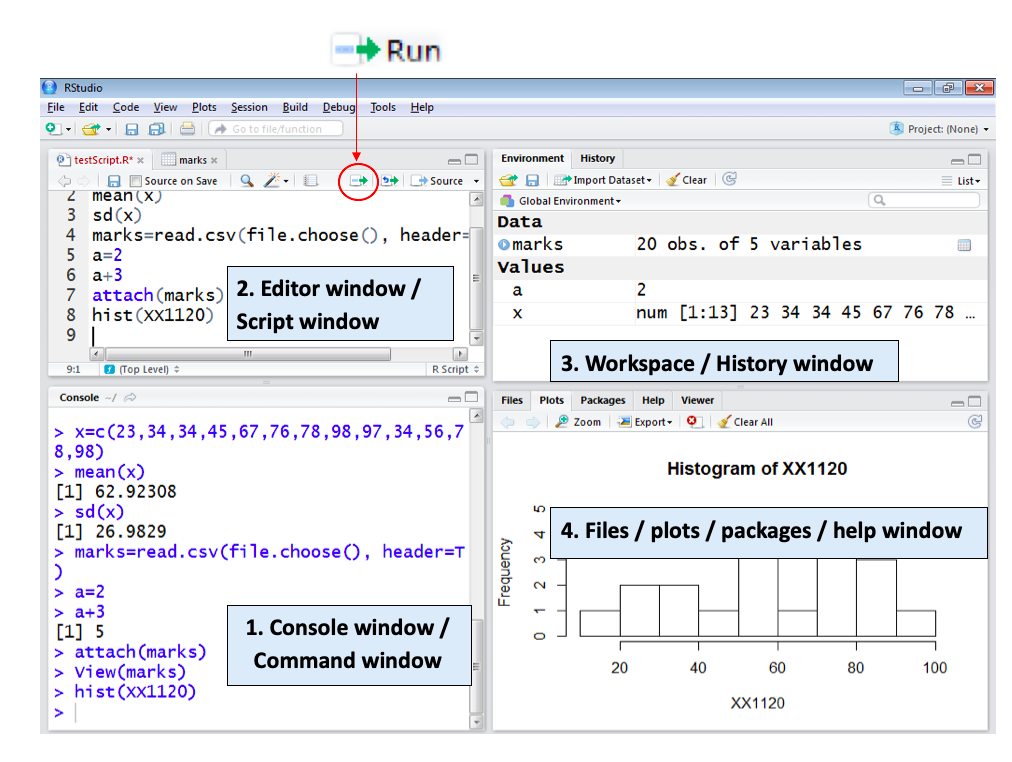
\includegraphics[width=0.9\linewidth]{figure/Rstudio1} \end{center}

\begin{center}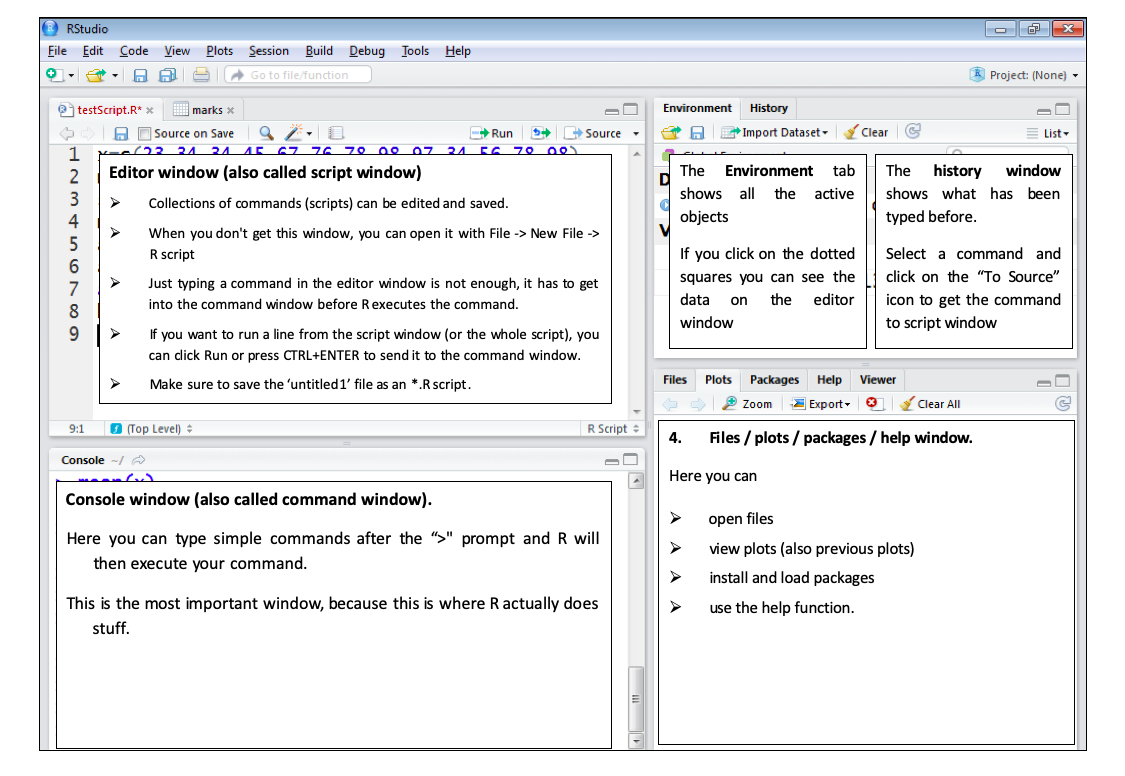
\includegraphics[width=0.9\linewidth]{figure/Rstudio2} \end{center}

Now you are familiar with the layout. Let's begin with R basics.

\hypertarget{installing-an-r-package}{%
\section{Installing an R Package}\label{installing-an-r-package}}

\begin{itemize}
\item
  The primary location for obtaining R packages is CRAN
\item
  Packages can be installed with the \texttt{install.packages()} function in R
\item
  To install a single package, pass the name of the package to the \texttt{install.packages()} function as the first argument
\end{itemize}

The following the code installs the \texttt{tidyverse} package from CRAN

\begin{Shaded}
\begin{Highlighting}[]
\KeywordTok{install.packages}\NormalTok{(}\StringTok{"tidyverse"}\NormalTok{)}
\end{Highlighting}
\end{Shaded}

\begin{itemize}
\item
  This command downloads the \texttt{tidyverse} package from CRAN and installs it on your computer
\item
  Any packages on which this package depends will also be downloaded and installed
\item
  \textbf{Installing the tidyverse package could take several minutes. You only need to do this once}.
\end{itemize}

\hypertarget{loading-an-r-packages}{%
\section{Loading an R Packages}\label{loading-an-r-packages}}

\begin{itemize}
\item
  Installing a package does not make it immediately available to you in R; you must load the package
\item
  The \texttt{library()} function is used to load packages into R
\item
  The following code is used to load the tidyverse package into R
\item
  \textbf{NOTE:} Do not put the package name in quotes!
\end{itemize}

\begin{Shaded}
\begin{Highlighting}[]
\KeywordTok{library}\NormalTok{(tidyverse)}
\end{Highlighting}
\end{Shaded}

\begin{itemize}
\tightlist
\item
  Some packages produce messages when they are loaded (but some don't)
\end{itemize}

\hypertarget{differentiation}{%
\chapter{Differentiation}\label{differentiation}}

First, we take the equation as an expression

\begin{Shaded}
\begin{Highlighting}[]
\NormalTok{f <-}\StringTok{ }\KeywordTok{expression}\NormalTok{(x}\OperatorTok{^}\DecValTok{2}\NormalTok{)}
\end{Highlighting}
\end{Shaded}

To calculate first derivative of \(f\), we use \texttt{D()} function and \texttt{x} to specify that derivation has to be carried out with respect to
\(x\).

\begin{Shaded}
\begin{Highlighting}[]
\NormalTok{f_}\DecValTok{1}\NormalTok{ <-}\StringTok{ }\KeywordTok{D}\NormalTok{(f, }\StringTok{"x"}\NormalTok{)}
\KeywordTok{print}\NormalTok{(f_}\DecValTok{1}\NormalTok{)}
\end{Highlighting}
\end{Shaded}

\begin{verbatim}
## 2 * x
\end{verbatim}

Sketch the graph of \(f\) and \(f^\prime\)

\begin{Shaded}
\begin{Highlighting}[]
\KeywordTok{library}\NormalTok{(ggplot2)}
\NormalTok{x <-}\StringTok{ }\KeywordTok{seq}\NormalTok{(}\OperatorTok{-}\DecValTok{1}\NormalTok{, }\DecValTok{1}\NormalTok{, }\DataTypeTok{by =} \FloatTok{0.1}\NormalTok{)}
\NormalTok{y <-}\StringTok{ }\KeywordTok{eval}\NormalTok{(f)}
\NormalTok{x <-}\StringTok{ }\KeywordTok{seq}\NormalTok{(}\OperatorTok{-}\DecValTok{1}\NormalTok{, }\DecValTok{1}\NormalTok{, }\DataTypeTok{by =} \FloatTok{0.1}\NormalTok{)}
\NormalTok{y1 <-}\StringTok{ }\KeywordTok{eval}\NormalTok{(f_}\DecValTok{1}\NormalTok{)}
\NormalTok{data <-}\StringTok{ }\KeywordTok{data.frame}\NormalTok{(x, y, y1)}
\KeywordTok{head}\NormalTok{(data)}
\end{Highlighting}
\end{Shaded}

\begin{verbatim}
##      x    y   y1
## 1 -1.0 1.00 -2.0
## 2 -0.9 0.81 -1.8
## 3 -0.8 0.64 -1.6
## 4 -0.7 0.49 -1.4
## 5 -0.6 0.36 -1.2
## 6 -0.5 0.25 -1.0
\end{verbatim}

\begin{Shaded}
\begin{Highlighting}[]
\NormalTok{p <-}\StringTok{ }\KeywordTok{ggplot}\NormalTok{(data, }\KeywordTok{aes}\NormalTok{(}\DataTypeTok{x =}\NormalTok{ x, }\DataTypeTok{y =}\NormalTok{ y)) }\OperatorTok{+}
\StringTok{  }\KeywordTok{geom_line}\NormalTok{()}
\KeywordTok{print}\NormalTok{(p)}
\end{Highlighting}
\end{Shaded}

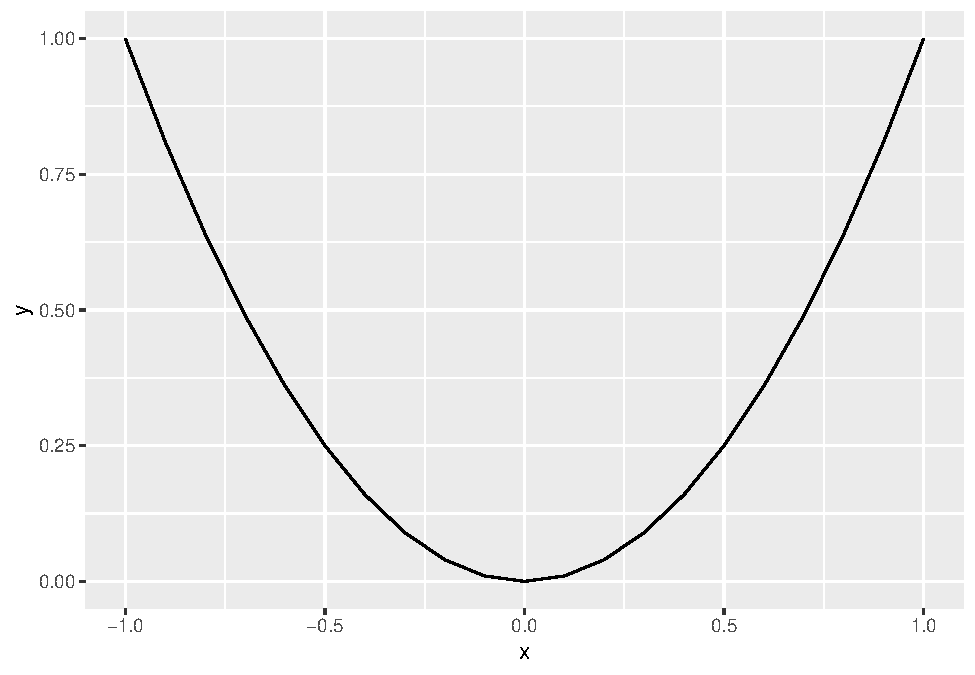
\includegraphics{bookdown-demo_files/figure-latex/unnamed-chunk-7-1.pdf}

\begin{Shaded}
\begin{Highlighting}[]
\NormalTok{q <-}\StringTok{ }\KeywordTok{ggplot}\NormalTok{(data, }\KeywordTok{aes}\NormalTok{(}\DataTypeTok{x =}\NormalTok{ x, }\DataTypeTok{y =}\NormalTok{ y1)) }\OperatorTok{+}
\StringTok{  }\KeywordTok{geom_line}\NormalTok{()}
\KeywordTok{print}\NormalTok{(q)}
\end{Highlighting}
\end{Shaded}

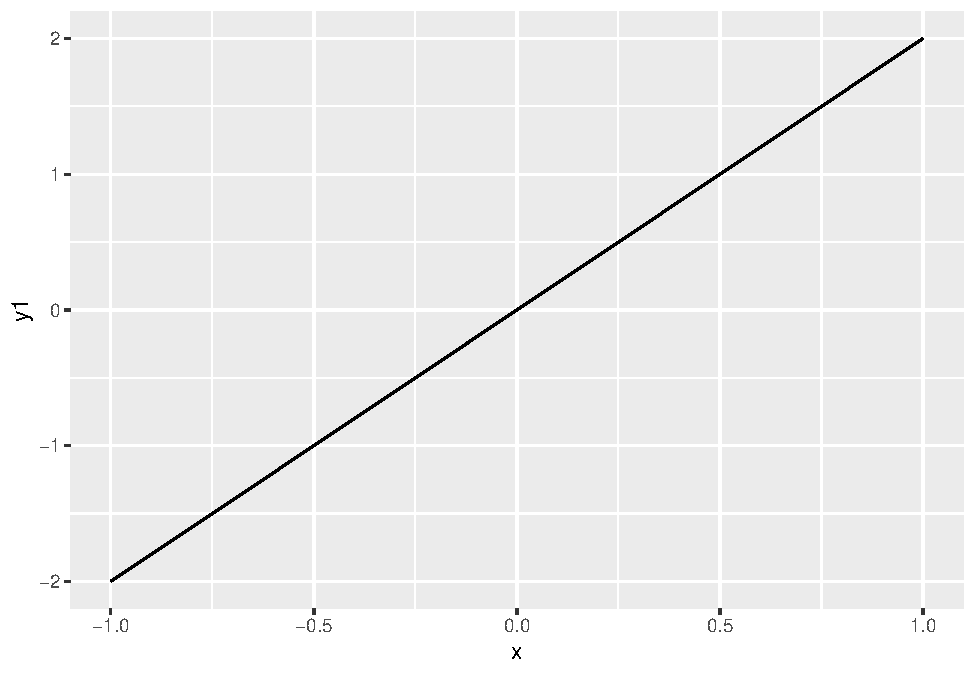
\includegraphics{bookdown-demo_files/figure-latex/unnamed-chunk-8-1.pdf}

\hypertarget{higher-derivatives}{%
\section{Higher Derivatives}\label{higher-derivatives}}

The following R command can be used to find second derivative of the above \(f\).

\begin{Shaded}
\begin{Highlighting}[]
\NormalTok{f_}\DecValTok{2}\NormalTok{ <-}\StringTok{ }\KeywordTok{D}\NormalTok{(}\KeywordTok{D}\NormalTok{(f, }\StringTok{"x"}\NormalTok{), }\StringTok{"x"}\NormalTok{)}
\KeywordTok{print}\NormalTok{(f_}\DecValTok{2}\NormalTok{)}
\end{Highlighting}
\end{Shaded}

\begin{verbatim}
## [1] 2
\end{verbatim}

\begin{Shaded}
\begin{Highlighting}[]
\NormalTok{x <-}\StringTok{ }\KeywordTok{seq}\NormalTok{(}\OperatorTok{-}\DecValTok{1}\NormalTok{, }\DecValTok{1}\NormalTok{, }\DataTypeTok{by =} \FloatTok{0.1}\NormalTok{)}
\NormalTok{y2 <-}\StringTok{ }\KeywordTok{eval}\NormalTok{(f_}\DecValTok{2}\NormalTok{)}

\NormalTok{data <-}\StringTok{ }\KeywordTok{data.frame}\NormalTok{(x, y, y1, y2)}
\KeywordTok{head}\NormalTok{(data)}
\end{Highlighting}
\end{Shaded}

\begin{verbatim}
##      x    y   y1 y2
## 1 -1.0 1.00 -2.0  2
## 2 -0.9 0.81 -1.8  2
## 3 -0.8 0.64 -1.6  2
## 4 -0.7 0.49 -1.4  2
## 5 -0.6 0.36 -1.2  2
## 6 -0.5 0.25 -1.0  2
\end{verbatim}

\begin{Shaded}
\begin{Highlighting}[]
\NormalTok{p <-}\StringTok{ }\KeywordTok{ggplot}\NormalTok{(data, }\KeywordTok{aes}\NormalTok{(}\DataTypeTok{x =}\NormalTok{ x, }\DataTypeTok{y =}\NormalTok{ y)) }\OperatorTok{+}
\StringTok{  }\KeywordTok{geom_line}\NormalTok{()}
\KeywordTok{print}\NormalTok{(p)}
\end{Highlighting}
\end{Shaded}

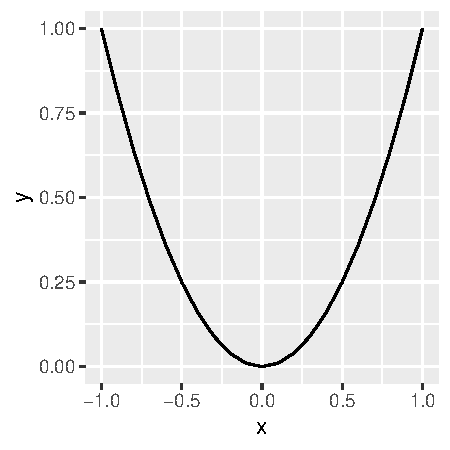
\includegraphics{bookdown-demo_files/figure-latex/unnamed-chunk-10-1.pdf}

\begin{Shaded}
\begin{Highlighting}[]
\NormalTok{q <-}\StringTok{ }\KeywordTok{ggplot}\NormalTok{(data, }\KeywordTok{aes}\NormalTok{(}\DataTypeTok{x =}\NormalTok{ x, }\DataTypeTok{y =}\NormalTok{ y1)) }\OperatorTok{+}
\StringTok{  }\KeywordTok{geom_line}\NormalTok{(}\DataTypeTok{colour =} \StringTok{"red"}\NormalTok{)}
\KeywordTok{print}\NormalTok{(q)}
\end{Highlighting}
\end{Shaded}

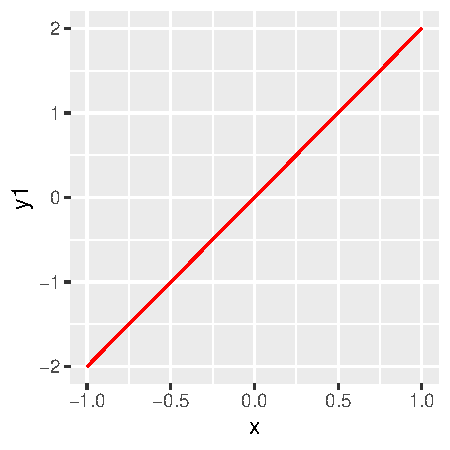
\includegraphics{bookdown-demo_files/figure-latex/unnamed-chunk-10-2.pdf}

\begin{Shaded}
\begin{Highlighting}[]
\NormalTok{r <-}\StringTok{ }\KeywordTok{ggplot}\NormalTok{(data, }\KeywordTok{aes}\NormalTok{(}\DataTypeTok{x =}\NormalTok{ x, }\DataTypeTok{y =}\NormalTok{ y2)) }\OperatorTok{+}
\StringTok{  }\KeywordTok{geom_line}\NormalTok{(}\DataTypeTok{colour =} \StringTok{"blue"}\NormalTok{)}
\KeywordTok{print}\NormalTok{(r)}
\end{Highlighting}
\end{Shaded}

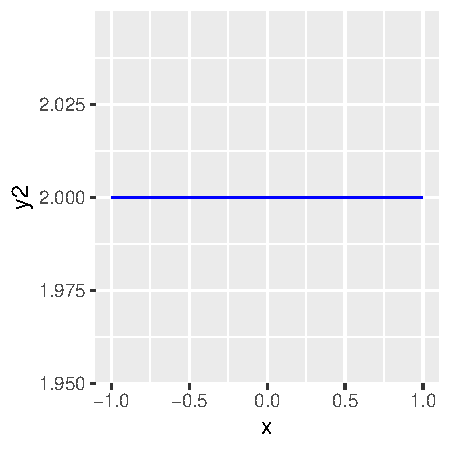
\includegraphics{bookdown-demo_files/figure-latex/unnamed-chunk-10-3.pdf}

\hypertarget{partial-derivatives}{%
\section{Partial Derivatives}\label{partial-derivatives}}

If the expression is having more than one independent variable, we can calculate differentiation with respect to each of them.

\begin{Shaded}
\begin{Highlighting}[]
\NormalTok{f <-}\StringTok{ }\KeywordTok{expression}\NormalTok{(x}\OperatorTok{^}\DecValTok{2} \OperatorTok{+}\StringTok{ }\NormalTok{y}\OperatorTok{^}\DecValTok{2}\NormalTok{)}

\NormalTok{x <-}\StringTok{ }\NormalTok{y <-}\StringTok{ }\KeywordTok{seq}\NormalTok{(}\OperatorTok{-}\DecValTok{3}\NormalTok{, }\DecValTok{3}\NormalTok{, }\DataTypeTok{length =} \DecValTok{20}\NormalTok{)}
\NormalTok{surface <-}\StringTok{ }\ControlFlowTok{function}\NormalTok{(x, y) \{}
  \KeywordTok{eval}\NormalTok{(f)}
\NormalTok{\}}
\NormalTok{z <-}\StringTok{ }\KeywordTok{outer}\NormalTok{(x, y, surface)}
\KeywordTok{persp}\NormalTok{(x, y, z)}
\end{Highlighting}
\end{Shaded}

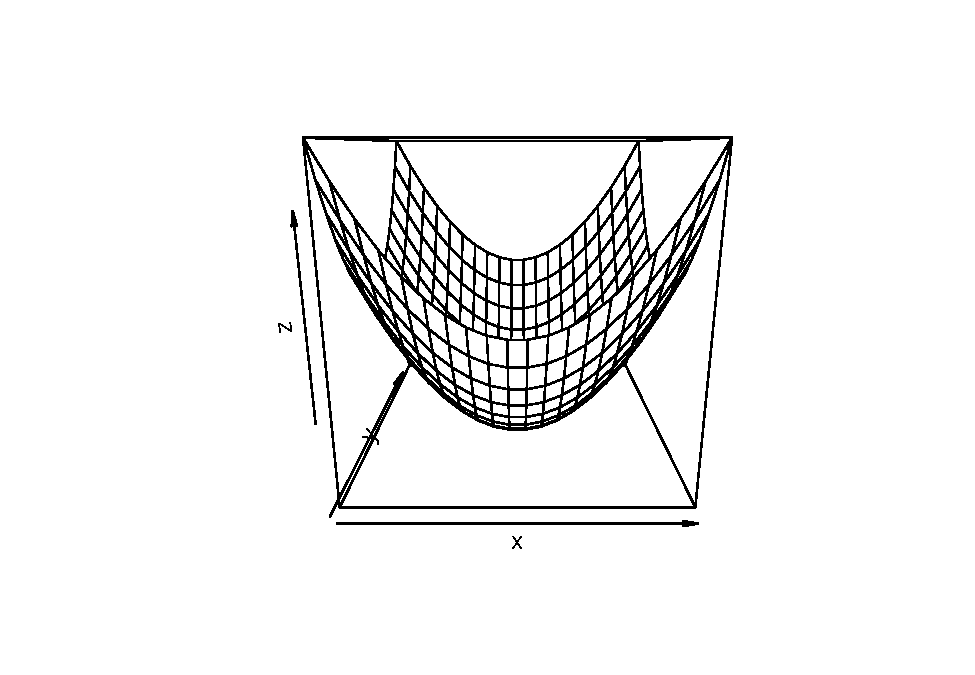
\includegraphics{bookdown-demo_files/figure-latex/unnamed-chunk-11-1.pdf}

Differentiate with respect to \texttt{x}

\begin{Shaded}
\begin{Highlighting}[]
\KeywordTok{D}\NormalTok{(f, }\StringTok{"x"}\NormalTok{)}
\end{Highlighting}
\end{Shaded}

\begin{verbatim}
## 2 * x
\end{verbatim}

Differentiate with respect to \texttt{y}

\begin{Shaded}
\begin{Highlighting}[]
\KeywordTok{D}\NormalTok{(f, }\StringTok{"y"}\NormalTok{)}
\end{Highlighting}
\end{Shaded}

\begin{verbatim}
## 2 * y
\end{verbatim}

\hypertarget{statistical-distributions}{%
\chapter{Statistical Distributions}\label{statistical-distributions}}

\hypertarget{applications}{%
\chapter{Applications}\label{applications}}

\hypertarget{final-words}{%
\chapter{Final Words}\label{final-words}}

We have finished a nice book.

\bibliography{book.bib,packages.bib}

\end{document}
